% !TeX document-id = {f19fb972-db1f-447e-9d78-531139c30778}
% !BIB program = biber
\documentclass[compress]{beamer}
\usepackage[T1]{fontenc}
\usepackage{pifont}
\usetheme[block=fill,subsectionpage=progressbar,sectionpage=progressbar]{metropolis} 

\usepackage{wasysym}
\usepackage{etoolbox}
\usepackage[utf8]{inputenc}

\usepackage{threeparttable}
\usepackage{subcaption}

\usepackage{tikz-qtree}
\setbeamercovered{still covered={\opaqueness<1->{5}},again covered={\opaqueness<1->{100}}}


\usepackage{listings}

\lstset{
	basicstyle=\scriptsize\ttfamily,
	columns=flexible,
	breaklines=true,
	numbers=left,
	%stepsize=1,
	numberstyle=\tiny,
	backgroundcolor=\color[rgb]{0.85,0.90,1}
}



\lstnewenvironment{lstlistingoutput}{\lstset{basicstyle=\footnotesize\ttfamily,
		columns=flexible,
		breaklines=true,
		numbers=left,
		%stepsize=1,
		numberstyle=\tiny,
		backgroundcolor=\color[rgb]{.7,.7,.7}}}{}


\lstnewenvironment{lstlistingoutputtiny}{\lstset{basicstyle=\tiny\ttfamily,
		columns=flexible,
		breaklines=true,
		numbers=left,
		%stepsize=1,
		numberstyle=\tiny,
		backgroundcolor=\color[rgb]{.7,.7,.7}}}{}



\usepackage[american]{babel}
\usepackage{csquotes}
\usepackage[style=apa, backend = biber]{biblatex}
\DeclareLanguageMapping{american}{american-UoN}
\addbibresource{../../bdaca.bib}
\renewcommand*{\bibfont}{\tiny}

\usepackage{tikz}
\usetikzlibrary{shapes,arrows,matrix}
\usepackage{multicol}

\usepackage{subcaption}

\usepackage{booktabs}
\usepackage{graphicx}

\graphicspath{{../../pictures/}}

\makeatletter
\setbeamertemplate{headline}{%
	\begin{beamercolorbox}[colsep=1.5pt]{upper separation line head}
	\end{beamercolorbox}
	\begin{beamercolorbox}{section in head/foot}
		\vskip2pt\insertnavigation{\paperwidth}\vskip2pt
	\end{beamercolorbox}%
	\begin{beamercolorbox}[colsep=1.5pt]{lower separation line head}
	\end{beamercolorbox}
}
\makeatother



\setbeamercolor{section in head/foot}{fg=normal text.bg, bg=structure.fg}



\newcommand{\question}[1]{
	\begin{frame}[plain]
		\begin{columns}
			\column{.3\textwidth}
			\makebox[\columnwidth]{
				\includegraphics[width=\columnwidth,height=\paperheight,keepaspectratio]{mannetje.png}}
			\column{.7\textwidth}
			\large
			\textcolor{orange}{\textbf{\emph{#1}}}
		\end{columns}
\end{frame}}




\title[Big Data and Automated Content Analysis]{\textbf{Big Data \& Automated Content Analysis} \\ Week 8 -- Wednesday: »Basics of Machine Learning«}
\author[Damian Trilling]{Damian Trilling \\ ~ \\ \footnotesize{d.c.trilling@uva.nl \\@damian0604} \\ \url{www.damiantrilling.net}}
\date{31 March 2021}
\institute[UvA]{Afdeling Communicatiewetenschap \\Universiteit van Amsterdam}

\begin{document}
	
	\begin{frame}{}
		\titlepage
	\end{frame}
	
	\begin{frame}{Today}
		\tableofcontents
	\end{frame}
	
\begin{frame}[standout]
Today, the great overview.

Next weeks: Specific applications for content analysis.
\end{frame}
	

\section[Recap]{Recap: Top-down vs bottom-up}


\begin{frame}[plain]
\makebox[\linewidth]{
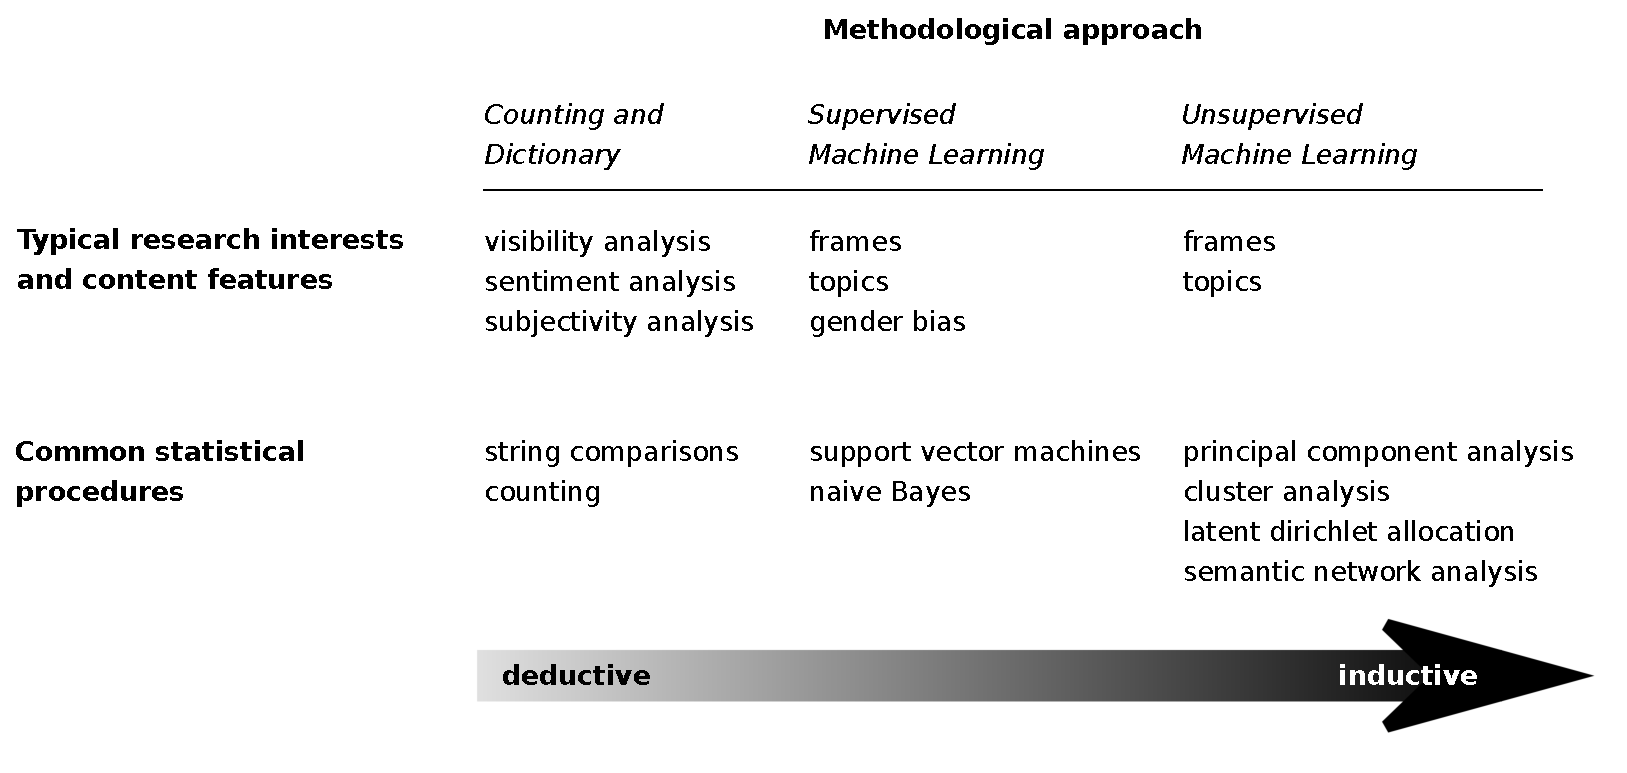
\includegraphics[width=\paperwidth,height=\paperheight,keepaspectratio]{boumanstrilling2016}}
\cite{Boumans2016}
\pause

\textbf{\textcolor{orange}{The same logic applies to non-textual data!}}
\end{frame}
%}




\begin{frame}{Some terminology }
\begin{columns}[t]
\column{.5\textwidth}

\begin{block}<1-4>{Supervised machine learning}
You have a dataset with both predictor and outcome (independent and dependent variables; features and labels) --- a \emph{labeled} dataset.
\onslide<2>{
	\footnotesize{Think of regression: You measured \texttt{x1}, \texttt{x2}, \texttt{x3} and you want to predict \texttt{y}, which you also measured}}
\end{block}

\column{.5\textwidth}

\begin{block}<3->{Unsupervised machine learning}
You have no labels. \onslide<4>{(\footnotesize{You did not measure \texttt{y})}}\\
\onslide<5>{\textbf{Again, you already know some techniques to find out how \texttt{x1}, \texttt{x2},\ldots \texttt{x\_i} co-occur from other courses:} \begin{itemize}
		\item Principal Component Analysis (PCA) and Singular Value Decomposition (SVD)
		\item Cluster analysis
		\item Topic modelling (Non-negative matrix factorization and Latent Dirichlet Allocation)
		\item \ldots
	\end{itemize}
}
\end{block}

\end{columns}

\end{frame}


\begin{frame}{Let's distinguish four use cases\ldots}

\begin{enumerate}
\item Finding similar variables (dimensionality reduction) -- unsupervised
\item Finding similar cases (clustering) -- unsupervised
\item Predicting a continous variable (regression) -- supervised
\item Predicting group membership (classification) -- supervised
\end{enumerate}
\end{frame}


\begin{frame}[plain]
	\begin{table}[]
		\resizebox{\textwidth}{!}{%
			\begin{tabular}{lllllll}
				& x1 & x2 & x3 & x4 & x5 & y \\
				case1 & \ding{110}  & \ding{110}  & \ding{110}  & \ding{110}  & \ding{110} & \ding{110} \\
				case2 & \ding{110}  & \ding{110}  & \ding{110}  & \ding{110}  & \ding{110} & \ding{110}\\
				case3 & \ding{110}  & \ding{110}  & \ding{110}  & \ding{110}  & \ding{110} & \ding{110}\\
				case4 & \ding{110}  & \ding{110}  & \ding{110}  & \ding{110}  & \ding{110} & \ding{110}\\
			\end{tabular}%
		}
	\end{table}
\end{frame}



\begin{frame}[plain]
\begin{table}[]
\resizebox{\textwidth}{!}{%
\begin{tabular}{lllllll}
& \textcolor{orange}{x1} & x2 & \textcolor{orange}{x3}& \textcolor{blue}{x4} & \textcolor{blue}{x5} & \textcolor{gray}{(y)} \\
case1 & \textcolor{orange}{\ding{110}}  & \ding{110}  & \textcolor{orange}{\ding{110}}  & \textcolor{blue}{\ding{110}} & \textcolor{blue}{\ding{110}} & \textcolor{gray}{(\ding{110})} \\
case2 & \textcolor{orange}{\ding{110}}  & \ding{110}  & \textcolor{orange}{\ding{110}}  & \textcolor{blue}{\ding{110}} & \textcolor{blue}{\ding{110}} & \textcolor{gray}{(\ding{110})} \\
case3 & \textcolor{orange}{\ding{110}}  & \ding{110}  & \textcolor{orange}{\ding{110}}  & \textcolor{blue}{\ding{110}} & \textcolor{blue}{\ding{110}} & \textcolor{gray}{(\ding{110})} \\
case4 & \textcolor{orange}{\ding{110}}  & \ding{110}  & \textcolor{orange}{\ding{110}}  & \textcolor{blue}{\ding{110}} & \textcolor{blue}{\ding{110}} & \textcolor{gray}{(\ding{110})} \\
\end{tabular}%
}
\end{table}
Dimensionality reduction: finding similar variables (features)
\end{frame}


\begin{frame}[plain]
\begin{table}[]
\resizebox{\textwidth}{!}{%
\begin{tabular}{lllllll}
& x1 & x2 & x3 & x4 & x5 & \textcolor{gray}{(y)} \\
\textcolor{orange}{case1} & \textcolor{orange}{\ding{110}}  & \textcolor{orange}{\ding{110}}  &\textcolor{orange}{\ding{110}}  &\textcolor{orange}{\ding{110}}   & \textcolor{orange}{\ding{110}} & \textcolor{gray}{(\ding{110})} \\
\textcolor{blue}{case2} & \textcolor{blue}{\ding{110}}  & \textcolor{blue}{\ding{110}}  &\textcolor{blue}{\ding{110}}  &\textcolor{blue}{\ding{110}}   & \textcolor{blue}{\ding{110}} & \textcolor{gray}{(\ding{110})} \\
\textcolor{orange}{case3} & \textcolor{orange}{\ding{110}}  & \textcolor{orange}{\ding{110}}  &\textcolor{orange}{\ding{110}}  &\textcolor{orange}{\ding{110}}   & \textcolor{orange}{\ding{110}} & \textcolor{gray}{(\ding{110})} \\
\textcolor{orange}{case4} & \textcolor{orange}{\ding{110}}  & \textcolor{orange}{\ding{110}}  &\textcolor{orange}{\ding{110}}  &\textcolor{orange}{\ding{110}}   & \textcolor{orange}{\ding{110}} & \textcolor{gray}{(\ding{110})} \\
\end{tabular}%
}
\end{table}
Clustering: finding similar cases
\end{frame}



\begin{frame}[plain]
\begin{table}[]
\resizebox{\textwidth}{!}{%
\begin{tabular}{llllllll}
& x1 & x2 & x3 & x4 & x5 & $\rightarrow$ & \textcolor{orange}{y} \\
case1 & \ding{110}  & \ding{110}  & \ding{110}  & \ding{110}  & \ding{110} & $\rightarrow$ &\textcolor{orange}{\ding{110}}  \\
case2 & \ding{110}  & \ding{110}  & \ding{110}  & \ding{110}  & \ding{110} & $\rightarrow$ &\textcolor{orange}{\ding{110}} \\
case3 & \ding{110}  & \ding{110}  & \ding{110}  & \ding{110}  & \ding{110} & $\rightarrow$ &\textcolor{orange}{\ding{110}} \\
case4 & \ding{110}  & \ding{110}  & \ding{110}  & \ding{110}  & \ding{110} & $\rightarrow$ &\textcolor{orange}{\ding{110}} \\
&&&&&&& \\
new case & \ding{110}  & \ding{110}  & \ding{110}  & \ding{110}  & \ding{110} & $\rightarrow$ &\textbf{\textcolor{orange}{?}} \\
\end{tabular}%
}
Regression and classification: learn how to predict $y$.
\end{table}
\end{frame}




\begin{frame}[plain]
\textbf{Note, again, that the \ding{110} signs can be \emph{anything}}.
For us, often word counts or $tf\cdot$ idf scores ($x$) and, for supervised approaches, a topic, a sentiment, or similar ($y$). 

But it could also be pixel colors or clicks on links or anything else.
\begin{table}[]
	\resizebox{\textwidth}{!}{%
		\begin{tabular}{lllllll}
			& x1 & x2 & x3 & x4 & x5 & y \\
			case1 & \ding{110}  & \ding{110}  & \ding{110}  & \ding{110}  & \ding{110} & \ding{110} \\
			case2 & \ding{110}  & \ding{110}  & \ding{110}  & \ding{110}  & \ding{110} & \ding{110}\\
			case3 & \ding{110}  & \ding{110}  & \ding{110}  & \ding{110}  & \ding{110} & \ding{110}\\
			case4 & \ding{110}  & \ding{110}  & \ding{110}  & \ding{110}  & \ding{110} & \ding{110}\\
		\end{tabular}%
	}
\end{table}
\end{frame}


\section{Finding similar variables}

\subsection{An introduction to dimensionality reduction}

\begin{frame}{Dimensionality reduction}
dimensionality = the number of features we have



\begin{block}{(1) Explorative data analysis and visualization}
\begin{itemize}
\item No good way to visualize 10,000 dimensions (or even 4)
\end{itemize}
\end{block}

\pause


\begin{block}{(2) The curse of dimensionality}
More features means more data (good!), but:
\begin{itemize}
\item Too many features can lead to unfeasible computation times
\item We need more training cases to increase the likelihood that the possible combinations actually occur
\end{itemize}
\end{block}
\end{frame}



\begin{frame}[fragile]{Dimensionality reduction}

\begin{block}{First approach: feature selection}
\begin{itemize}
\item Only choose the features that are really relevant
\end{itemize}
\end{block}


Example of what we did before: Exclude all terms that occur in more than 50\% of the documents, or in less than $n=5$ documents:

\begin{lstlisting}
vec = CountVectorizer(max_df=0.5, min_df=5)
\end{lstlisting}

\tiny{\url{https://scikit-learn.org/stable/modules/generated/sklearn.feature\_extraction.text.CountVectorizer.html}}

\end{frame}





\begin{frame}[fragile]{Dimensionality reduction}

\begin{block}{Second approach: feature extraction}
\begin{itemize}
\item Create a smaller set of features
\item E.g.: 1,000 features $\rightarrow$ PCA to reduce to 50 components $\rightarrow$ SML with these 50 component scores as features
\end{itemize}
\end{block}

\end{frame}



\begin{frame}[fragile]{Dimensionality reduction}

So, we can use unsuvised ML as a dimension reduction step in a supervised ML pipeline. 

\vspace{0.5cm}
But it can also be a goal in itself, to understand the data better or to visualize them.
\end{frame}







\subsection{Principal Component Analysis and Singular Value Decomposition}


\begin{frame}{PCA}
\begin{itemize}
\item related to and often confused with Factor Analysis (same menu item in SPSS -- many people who believe they run FA actually run PCA!)
\item Components are ordered (first explains most variance)
\item Components do \emph{not} necessarily carry a meaningful interpretation
\end{itemize}
\end{frame}

\begin{frame}{PCA}
\makebox[\linewidth]{\includegraphics[width=\paperwidth,height=.6\paperheight,keepaspectratio]{pca}}

\tiny{\url{https://upload.wikimedia.org/wikipedia/commons/f/f5/GaussianScatterPCA.svg}}
\end{frame}


\begin{frame}[fragile,plain]{Running PCA}
	
Example of a PCA on a BOW representation of some texts:


\begin{lstlisting}
myvec = CountVectorizer(texts, max_df=.5, min_df=5)
mypca = PCA(n_components=2)

mypipe = make_pipeline(myvec, FunctionTransformer(lambda x: x.todense(), accept_sparse=True), mypca)

r = mypipe.fit_transform(texts)
\end{lstlisting}


\small{PCA does not accept a \textit{sparse matrix} as input (but the CountVectorizer gives one as output), so we need to transform it into a \textit{dense matrix}.}


\end{frame}



\begin{frame}[fragile,plain]{Plotting the result}
\begin{lstlisting}
plt.scatter([e[0] for e in r], [e[1] for e in r], alpha=.6)
\end{lstlisting}

\makebox[\linewidth]{\includegraphics[width=\paperwidth,height=.6\paperheight,keepaspectratio]{pca-example}}


\end{frame}



\begin{frame}[fragile]{Singular value decomposition}
The need to use a dense matrix is \emph{really} a problem for large feature sets (which we have in NLP).
\pause

We therefore can better use SVD, which is essentially* the same and very simple to use:

\begin{lstlisting}
mysvd = TruncatedSVD(n_components=2)
mypipe = make_pipeline(myvec, mysvd)
r = mypipe.fit_transform(texts)
\end{lstlisting}

\footnotesize{(In this specific case, we even get exactly the same plot\ldots)}


\footnotesize{
* It's mathematically different, but you can SVD is even used ``under the hood'' by several PCA modules to solve PCA problems.

More info and background: \url{https://towardsdatascience.com/pca-and-svd-explained-with-numpy-5d13b0d2a4d8}}

\end{frame}







\section{Finding similar cases}

\subsection{k-means clustering}




\begin{frame}{Grouping features vs grouping cases}
Let's consider a corpus of several thousand user comments.

We could use SVD or similar techniques to 
\begin{itemize}
\item figure out relationships between features
\item see which features stand out
\item get a first sense what topics are in the corpus.
\end{itemize}
\pause

But:
\begin{itemize}
\item<+-> We do not learn anything about \emph{which} texts (cases) belong to which topic
\item<+-> We could use the component scores returned by \texttt{.fit\_transform()} to then group our cases
\end{itemize}

\pause 
$\Rightarrow$ \textbf{Alternative: Choose the opposite approach and first find out which cases are most similar, \textit{then} describe what features characterize each group of cases}


\end{frame}




\begin{frame}{k-means clustering}
\begin{itemize}[<+->]
\item Goal: group cases into $k$ clusters
\item $k$ is set in advance
\item Algorithm to determine \textit{k} centroids (points in the middle of the cases that belong to it) such that the distances between the cases and their centroids are minimized
\item non-deterministic: starts with a randomly choosen centroids (there are other versions)
\item Cheap to compute: works even with large number of cases
\item We can run PCA first to reduce the number of features if we want/need to
\end{itemize}
\end{frame}




\begin{frame}{k-means clustering}
\makebox[\linewidth]{\includegraphics[width=\paperwidth,height=.65\paperheight,keepaspectratio]{kmeans}}

{\tiny{\url{https://upload.wikimedia.org/wikipedia/commons/e/ea/K-means\_convergence.gif}}}

Notice the big symbols indicating the centroids.
\end{frame}


\begin{frame}[plain,fragile]
\begin{lstlisting}
from sklearn.feature_extraction.text import TfidfVectorizer
from sklearn.cluster import KMeans

k = 5
texts = ['text1 ejkh ek ekh', 'ekyerykel'] # a list of texts

vec = TfidfVectorizer(min_df=5, max_df=.4)
features = vec.fit_transform(texts)
km = KMeans(n_clusters=k, init='k-means++', max_iter=100, n_init=1)
predictions = km.fit_predict(features)

\end{lstlisting}

That's it!
\pause

\begin{itemize}
\item \texttt{predictions} is a list of integers indicated the predicted cluster number. We can thus use \texttt{zip(predictions, texts)} to put them together.
\item<+-> We could also use \texttt{.fit()} and \texttt{.transform()} sperately and use our \texttt{km} to predict clusters for additional cases we have not used to train the model
\end{itemize}

\end{frame}


\begin{frame}[fragile,plain]{Let's get the terms closest to the centroids}
\begin{lstlisting}
order_centroids = km.cluster_centers_.argsort()[:, ::-1]
terms = vec.get_feature_names()

print("Top terms per cluster:")

for i in range(k):
    print("Cluster {}: ".format(i), end='')
    for ind in order_centroids[i, :10]:
        print("{} ".format(terms[ind]), end='')
        print()
\end{lstlisting}
\pause
returns something like:

\begin{lstlisting}
Top terms per cluster:
Cluster 0: heard could if opinions info day how really just around 
Cluster 1: systems would ken pc am if as care summary ibm 
Cluster 2: year car years was my no one higher single than 
Cluster 3: which like seen 1000 few easily based personal work used 
Cluster 4: as was he if they my all will get has 
\end{lstlisting}
\end{frame}


\begin{frame}{Using k-means clustering\ldots}
\begin{itemize}
\item we get the cluster membership for each text; and
\item we get the terms that are most characteristic for the documents in each cluster.
\end{itemize}
\end{frame}

\begin{frame}{Finding the optimal $k$}

\begin{itemize}
\item The only way to find $k$ is to estimate multiple models with different $k$s
\item No single best solution; finding a balance between error within clusters (distances from centroid) and low number of clusters.
\item An elbow plot can be helpful 
\end{itemize}


\end{frame}


\subsection{Hierarchical clustering}


\begin{frame}{Downsides of k-means clustering}
k-means is fast, but has problems:

\begin{itemize}
\item $k$ can only be determined by fitting multiple models and comparing them
\item bad results if the wrong $k$ is chosen
\item bad results if the (real) clusters are non-spherical
\item bad results if the (real) clusters are not evenly sized
\end{itemize}
\end{frame}


\begin{frame}{Hiearchical clusttering}
\begin{block}{General idea}
\begin{itemize}
\item To start, each case has its own cluster
\item Merge the two clusters that are most similar
\item Repeat until desired number of clusters is reached
\end{itemize}

\end{block}

\pause

\begin{block}{Different options}
\begin{itemize}
\item Stopping criterion: based on numerical statistic (e.g., Duda-Hart) or dendrogram
\item Linkage: how to determine which two clusters should be merged?
\end{itemize}

\end{block}
\end{frame}


\begin{frame}{Let's look into some options}

\url{https://scikit-learn.org/stable/modules/clustering.html\#hierarchical-clustering}

$\Rightarrow$ Ward's linkage is a good default all-rounder choice, especially if you encounter the problem that other linkages lead to almost all cases ending up in one cluster. 
\end{frame}


\begin{frame}{Hierarchical clustering takeaway}
\begin{itemize}
\item The main reason \emph{not} to use hierarchical methods (but k-means) is their computational cost: when clustering survey data of media users, never use $k$-means!
\item But for NLP/ML, costs may be too high (if not used carefully)
\item Very much worth considering, though, if you are really into grouping cases!
\end{itemize}
\end{frame}


%\section{Important notes}



\begin{frame}{Important notes for all techniques}
\begin{block}{Consider the scales of measurement}
Clustering is based on distances -- if your features are not measured on the same scale, or if it is not meaningful to calculate a numerical distance, it won't produce meaningful results!

Consider standardizing/whitening your features!
\end{block}

\pause

\begin{block}{Pay attention outliers/extreme cases}
Extreme cases or outliers can have a strong influence.
\end{block}

\pause 
\begin{block}{Do proper pre-processing}
To reduce the number of features, but also to have \emph{meaningful} features (dimensions on which you expect high distances between the clusters).
\end{block}


\end{frame}


\section{Predicting things}






\subsection{You have done it before!}
\begin{frame}{You have done it before!}
	\begin{block}{Regression}<2->
		\begin{enumerate}
			\item<3-> Based on your data, you estimate some regression equation 	$y_i = \alpha + \beta_1 x_{i1} + \cdots + \beta_p x_{ip} + \varepsilon_i$
			\item<4-> Even if you have some \emph{new unseen data}, you can estimate your expected outcome $\hat{y}$!
			\item<5-> Example: You estimated a regression equation where $y$ is newspaper reading in days/week: $y = -.8 + .4 \times man + .08 \times age$
			\item<6-> You could now calculate $\hat{y}$ for a man of 20 years and a woman of 40 years -- \emph{even if no such person exists in your dataset}: \\
			$\hat{y}_{man20} = -.8 + .4 \times 1 + .08 \times 20 = 1.2$ \\
			$\hat{y}_{woman40} = -.8 + .4 \times 0 + .08 \times 40 = 2.4$
		\end{enumerate}
	\end{block}	
	
\end{frame}



\begin{frame}{}
	\huge{This is\\ Supervised Machine Learning!}
\end{frame}

\begin{frame}{\ldots but\ldots}
	\begin{itemize}
		\item<1-> We will only use \emph{half} {\tiny{(or another fraction)}} of our data to estimate the model, so that we can use the other half to check if our predictions match the manual coding (``labeled data'',``annotated data'' in SML-lingo)
		\begin{itemize}
			\item<2->e.g., 2000 labeled cases, 1000 for training, 1000 for testing --- if successful, run on 100,000 unlabeled cases
		\end{itemize}
		\item<3-> We use many more independent variables (``features'')
		\item<4-> Typically, IVs are word frequencies (often weighted, e.g. tf$\times$idf) ($\Rightarrow$BOW-representation)
	\end{itemize}
\end{frame}


\subsection{From regression to classification}
	
\begin{frame}[standout]
In the machine learning world, predicting some continous value is referred to as a \textcolor{orange}{regression} task. If we want to predict a binary or categorical variable, we call it a \textcolor{orange}{classification} task.

(quite confusingly, even if we use a logistic regression for the latter)
\end{frame}


\begin{frame}{Classification tasks}
For many computational approaches, we are actually not that interested in predicting a continous value. Typical questions include:
\begin{itemize}
	\item Is this article about topix A, B, C, D, or E?
	\item Is this review positive or negative?
	\item Does this text contain frame F?
	\item I this satire? 
	\item Is this misinformation?
	\item Given past behavior, can I predict the next click?
\end{itemize}
\end{frame}



\begin{frame}[plain]
	\begin{columns}[]
		\column{.5\textwidth}
		
		{\tiny{http://commons.wikimedia.org/wiki/File:Precisionrecall.svg}}
		\makebox[\linewidth]{
			\includegraphics[width=\paperwidth,height=\paperheight,keepaspectratio]{../pictures/precisionrecall.png}}
		
		\column{.5\textwidth}
		\begin{block}{Some measures}
			\begin{itemize}
				\item Accuracy
				\item Recall
				\item Precision
				\item $\text{F1}=2\cdot \frac{\text{precision}\cdot \text{recall}}{\text{precision}+\text{recall}}$
				\item AUC (Area under curve) $[0,1]$, $0.5=$ random guessing
			\end{itemize}
		\end{block}
		
		
	\end{columns}
	
\end{frame}





\begin{frame}{Different classification algorithms}

\begin{itemize}[<+->]
	\item It is an empirical question which one works best
	\item We typically try several ones and select the best
	\item (remember: we have a test dataset that we did \emph{not} use to train the model, so that we can assess how well it predicts the test labels based on the test features)
	\item To avoid $p$-hacking-like scenario's (which we call ``overfitting''), there are techniques available (cross-validation, later in this course)
\end{itemize}
(to make it easier, imagine a binary classfication ("positive"/"negative"), but it doesn't really matter whether there are two or more labels)
\end{frame}






\begin{frame}{Naïve Bayes}
	\begin{block}{Bayes' theorem}
		$$ P(A \mid B) = \frac{P(B \mid A) \times P(A)}{P(B)} $$
	\end{block}
	\pause
	\textcolor{red}{A = Text is about sports\\
		B = Text contains `very', `close', `game'}.
	\pause
	Furthermore, we simply multiply the propabilities for the features:
	\textcolor{red}{$$P(B) = P(very\, close\, game) = P(very) \times P(close) \times P(game)$$}
	We can fill in all values by counting how many articles are about sports, and how often the words occur in these texts.
	\vspace{0.3cm}
	\footnotesize{
		(Fully elaborated example on \url{https://monkeylearn.com/blog/practical-explanation-naive-bayes-classifier/})}
\end{frame}

\begin{frame}{Naïve Bayes}
	\begin{itemize}[<+->]
		\item It's ``naïve'' because the features are treated as completely independent ($\neq$ ``controlling'' in regression analysis)
		\item It's fast and easy
		\item It's a good \emph{baseline} for binary classification problems
	\end{itemize}
\end{frame}




\begin{frame}{Na\"ive Bayes}
$$ P(\rm{label} \mid \rm{features}) =$$
$$ \frac{P(x_1 \mid label) \cdot P(x_2 \mid \rm{label})\ \cdot P(x_3 \mid label) \cdot P(label)}{P(x_1) \cdot P(x_2) \cdot P(x_3)}$$.

	
\begin{itemize}
	\item Formulas always look intimidating, but we only need to fill in how many documents containing feature $x_n$ have the label, how often the label occurs, and how often each feature occurs
	\item Also for computers, this is \emph{really easy and fast}
	\item Weird assumption: features are independent
	\item Often used as a baseline
\end{itemize}
\end{frame}




\begin{frame}{Logistic Regression}
	\begin{block}{Probability of a binary outcome in a regression model}
		$$p = \frac{1}{1 + e^{-(\beta_0 + \beta_1 x_1 + \beta_2 x_2 + \ldots + \beta_n x_n)}}$$
	\end{block}
	Just like in OLS regression, we have an intercept and regression coefficients. 
	We use a threshold (default: 0.5) and above, we assign the positive label (`good movie'), below, the negative label (`bad movie').
\end{frame}
\begin{frame}{Logistic Regression}
	\begin{itemize}[<+->]
		\item The features are \emph{not} independent.
		\item Computationally more expensive than Naïve Bayes
		\item We can get probabilities instead of just a label
		\item That allows us to say how sure we are for a specific case
		\item \ldots or to change the threshold to change our precision/recall-tradeoff
	\end{itemize}
\end{frame}

\begin{frame}{Support Vector Machines}
	\begin{columns}
		\column{.5\linewidth}
		\begin{itemize}
			\item	Idea: Find a hyperplane that best seperates your cases
			\item Can be linear, but does not have to be (depends on the so-called kernel you choose)
			\item Very popular 
		\end{itemize}
		\column{.5\linewidth}	
		\includegraphics[width=.8\linewidth,height=.5\paperheight,keepaspectratio]{../pictures/svm}
		\tiny{\url{https://upload.wikimedia.org/wikipedia/commons/b/b5/Svm\_separating\_hyperplanes\_\%28SVG\%29.svg}}
	\end{columns}
	\vfill
	\footnotesize{(Further reading: \url{https://monkeylearn.com/blog/introduction-to-support-vector-machines-svm/)}}
\end{frame}

\begin{frame}{SVM vs logistic regression}
\begin{itemize}
	\item for \emph{linearly separable} classes not much difference
	\item with the right hyperparameters, SVM is less sensitive to outliers
	\item biggest advantage: with the \emph{kernel trick}, data can be transformed that they \emph{become} linearily separable
\end{itemize}
\end{frame}


\begin{frame}{Decision Trees and Random Forests}
	\begin{columns}
		\column{.5\linewidth}
		\begin{itemize}[<+->]
			\item Model problem as a series of decisions (e.g., if cloudy then \ldots if temperature > 30 degrees then \ldots)
			\item Order and cutoff-points are determined by an algorithm
			\item Big advantage: Model non-linear relationships
			\item And: They are easy to interpret (!) (``white box'')
		\end{itemize}
		\column{.5\linewidth}	
		\includegraphics[width=.8\linewidth,height=.5\paperheight,keepaspectratio]{../pictures/decisiontree}
		\tiny{\url{https://upload.wikimedia.org/wikipedia/en/4/4f/GEP\_decision\_tree\_with\_numeric\_and\_nominal\_attributes.png}}
	\end{columns}
\end{frame}
\begin{frame}{Decision Trees and Random Forests}
	\begin{block}{Disadvantages of decision trees}
		\begin{itemize}
			\item comparatively inaccurate
			\item once you are in the wrong branch, you cannot go `back up'
			\item prone to overfitting (e.g., outlier in training data may lead to completely different outcome)
		\end{itemize}
	\end{block}
	\pause
	Therfore, nowadays people use \emph{random forests}: Random forests \emph{combine} the predictions of \emph{multiple} trees
	$\Rightarrow$ might be a good choice for your non-linear classification problem
\end{frame}









\section{Summing up}

\question{Any questions?}

\begin{frame}{Things to remember}
\begin{itemize}
	\item unsupervised vs supervised
	\item rough understanding of different techniques and when to use them
	\item evaluation metrics (e.g., precision, recall)
\end{itemize}
$\Rightarrow$ Practical implementations will come in the next weeks.

\textbf{Enjoy the Easter break!}
\end{frame}

\begin{frame}[plain]
	\printbibliography
\end{frame}


\end{document}